\documentclass{standalone}
\usepackage{tikz}
%\usetikzlibrary{positioning,shapes}
\usepackage{pgfplots}
\begin{document}
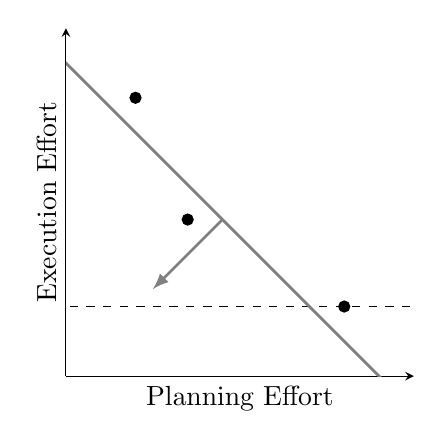
\begin{tikzpicture}
\tikzset{>=latex} % arrow heads

\begin{axis}[
   xlabel=Planning Effort,
   ylabel=Execution Effort,
   ylabel near ticks,
   xlabel near ticks,
   ticks=none,
   axis lines=left,
   xmin=0,xmax=1,
   ymin=0,ymax=1,
   width=6cm, height=6cm]
   
\addplot[mark=none,dashed] {0.2};

\addplot[mark=none,color=black!50,line width=1pt] {0.9 - x};
\draw[->,color=black!50,line width=1pt] (axis cs:0.45,0.45) -- (axis cs:0.25,0.25);

\addplot[mark=*] plot coordinates { (0.8, 0.2) };

\addplot[mark=*] plot coordinates { (0.2, 0.8) };

\addplot[mark=*] plot coordinates { (0.35, 0.45) };

\end{axis}

\end{tikzpicture}
\end{document}
